% !TeX program = xelatex
% !TeX encoding = UTF-8
\documentclass[UTF8]{standalone}
\usepackage{amsmath,fourier,esint,ctex,tikz}
\begin{document}
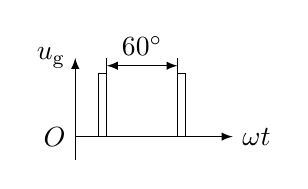
\begin{tikzpicture}
	\draw[-latex] (0,0) node[left] {$O$} -- (2,0) node[right] {$\omega t$};
	\draw[-latex] (0,-0.3) -- (0,1) node[left] {$u_{\mathrm{g}}$};
	\coordinate (a) at (0.3,0);
	\coordinate (b) at (1.3,0);
	\draw (a) rectangle ++ (0.1,0.8);
	\draw (b) rectangle ++ (0.1,0.8);
	\draw (a) ++ (0.1,0.8) -- ++ (0,0.2);
	\draw (b) ++ (0,0.8) -- ++ (0,0.2);
	\draw[latex-latex] (a) ++ (0.1,0.9) -- node[above] {$60^\circ$} ++ (0.9,0);
\end{tikzpicture}
\end{document}